%!TEX program = xelatex
%!TEX TS-program = xelatex
%!TEX encoding = UTF-8 Unicode

\documentclass[12pt, a4paper]{article} % A4 纸,字体大小为 12pt 的 article 类文档
\usepackage{CJKutf8} % 中文支持
\usepackage{graphicx} % 插入图片
\usepackage{subfigure} % 插入多图时用子图显示的宏包
\usepackage{listings} % 支持代码显示
\usepackage[colorlinks,linkcolor=blue]{hyperref} % 超链接
\usepackage{ulem} % 删除线
\usepackage{xcolor} % 定制颜色
\usepackage{caption2} % 浮动图形和表格标题样式
\usepackage{amssymb} % 数学符号
\usepackage{indentfirst} % 中文段落首行缩进
\usepackage{tikz} % 画图
\usepackage{pgfplots} % 画图
\usepackage{amsmath} % 处理数学公式
\usepackage{mathtools} % 处理数学公式
\setlength{\parskip}{0.5em} % 段落间距
\renewcommand{\figurename}{图} % 将图表的标题设置为中文“图”
\usetikzlibrary{tikzmark,calc,decorations.pathreplacing} % tikzmark 用于标记位置,calc 用于计算,decorations.pathreplacing 用于画大括号


\title{第二十三·合作博弈 · 效率、公平与团体理性}
\author{hoochanlon}
\date{\today}

\begin{document}
	\begin{CJK*}{UTF8}{gbsn}
		\maketitle
        \clearpage
        \section{塔木德的妇女部婚卷}
        《塔木德·妇女部·婚卷》名富翁在婚书中向他的三位妻子许诺,死后将给A老婆100个金币,B老婆200个金币,C老婆300个金币。
        可是富翁死后人们发现他的遗产根本不到600个金币,那么三位妻子应怎么分配这位富翁的遗产呢? \par

        拉比的具体裁决方案:

        \begin{itemize}
            \item 只有100金币时,平均分配法100/3,100/3,100/3。
            \item 只有200金币时,神奇分配法50,75,75。
            \item 只有300金币时,按比例分配法50,100,150。
        \end{itemize}


        遗产分配需要满足的原则:

        \begin{itemize}
            \item 仅分割有争议财产,无争议财产不需要分割。
            \item 宣称拥有更多财产权利的一方,其最终所得不少于宣称拥有较少财产权利一方。
            \item 财产争议者超过两人时,将所有争议者按照其诉求金额排序,最小者自成一组,剩下所有争议者另成一组,争议财产在两组间公平分配。
        \end{itemize}

        这样分遗产的意义,当资源匮乏的时候能够保住弱势方的利益,当资源充足的时候,又有利于体现所有者的意愿。从而起到了兼顾的作用。根据这个原则,
        我们可以推导出任意遗产的分配结果:

        \begin{itemize}
            \item 若$N \leq 150$,ABC各得N/3。
            \item 若$150<N \leq 250$,A得50,B和C各得(N-50)/2。
            \item 若$250<N \leq 350$,A得50,B得100,C得到N-150。
            \item 若$350<N \leq 500$,A得50,B得(N/2)-75,C得(N/2)+25。
            \item 若$500<N<600$,A得(N/2)-200,B得(N/4)+50,C得(N/4)+150。
            \item 若N≥600,A得N/6,B得N/3,C得N/2。
        \end{itemize}

        \clearpage
        \section{合作博弈和非合作博弈}

        \subsection{合作博弈和非合作博弈区别}
        合作博弈与非合作博弈,两者的主要区别在于人们的行为互相作用时,当事人是否达成一个具有约束力的协议,如果有,就是合作博弈;没有,就是非合作博弈。
        非合作博弈模型强调的是个体理性,以个体利益最大化为原则;合作博弈强调的是群体理性,以实现群体利益最大化为目标。

        \subsection{合作博弈和非合作博弈联系}
        非合作博弈是参与者无法选择协调相互之间的策略选择的博弈,当其他参与者会对我的策略选择做出最优反应时,什么才是我的最佳策略选择。
        合作博弈是参与者可以协调相互之间策略选择的博弈,合作博弈主要解决如果参与者的策略可以相互协调,那么什么样的选择才会带来整体利益最大化。\par
        一般而言,承诺不可信,相互的协议就不可能达成,得到的往往是非合作博弈解。如果承诺可信,相互之间能达成有约束力的协议,得到的往往合作博弈解。
        由此,通过一个有约束力的协议,可以将非合作博弈转化为合作博弈,把原本不能实现的合作方案得以实现,每个参与者的收益都能得到提高,从而实现群体利益最大化。\par

        \subsection{合作博弈的基本概念}
        在合作博弈中,有许多不同于非合作博弈的概念体系,合作博弈的核心是参与人如何结盟,以及如何分配通过结盟产生的新增收益。
        每个参与者都能按照自己的利益和其他参与者组成一个小集团,彼此合作以谋求更大的利益。\par

        设:参与人为1- N,S为参与人的一个集合,$S \subseteq N$,$S \neq \emptyset$,$S \neq N$,$S \neq \{i\}$,$i \in N$。合作博弈的结果必须是帕累托改进,
        博弈各方的利益都有所增加,或至少有一部分参与者的利益有所增加,另一部分参与者利益不受损失。\par

        合作博弈必须能够产生出一种合作的剩余,那么至于合作剩余在各方怎么分配,取决于博弈各方的力量对比和制度设计。合作设计的分配,它既是合作的结果,
        又是达成合作的前提条件,因此更大联盟的总收益一定是大于较小联盟的收益。合作博弈强调群体理性,强调效率、公平和正义,要想强调群体利益最大化,
        就需要建立一个描述群体理性的特征函数。

        \begin{itemize}
            \item[] 给定一个N个参与人的合作博弈,特征函数v是从所有不同联盟(共2N个)到一个实数集的映射。
            \item[] v(S)是N中的联盟S和其他联盟(N-S)的最大期望收益,称为联盟S的特征函数。
        \end{itemize}

        特征函数是研究合作博弈的基础,决定特征函数的过程实际上就是分析合作博弈的过程。

        \clearpage
        \section{合作博弈的分析框架}
        非合作的博弈是纯粹个体之间的博弈,合作博弈是联盟之间的博弈,单个个体也被认为是联盟的一种,所以合作博弈也可以分析个体之间的博弈。特征函数是
        某个联盟与其他联盟博弈时所获得的最大收益,这是某个联盟是否与其他参与者结盟的决策基础。更大联盟的建立一定不能让参与联盟的人吃亏,合作收益可以在参与者之间自由转移(可转移效用)。\par

        在合作博弈中参与者的收益转让是与协议联系在一起的,联盟成员一般用支付货币的方式,来弥补参与者放弃单人联盟或其他联盟形式的预期损失(旁支付)。
        在允许旁支付的条件下,在确保每个参与者至少获得非合作博弈收益的基础上,那些能使总收益达到最大值的所有合作博弈联盟,构成合作博弈的解。
        如果存在两种或两种以上的有效配置方案时,那么所有的有效解的集合构成的解集(全部有效)的帕累托最优的联盟结构和收益分配方式的集合,
        参与者至少能够获得非合作博弈下的收益。\par

        合作博弈中的核(包含所有使团体中的任何成员,都不能从联盟重组中获益的配置方案)。合作博弈的核可以是任意的,也可以一种或多种联盟结构,而
        没有核的联盟结构,我们称作“空核博弈”。合作博弈的解集由全部有效策略组合与旁支付构成,旁支付保证每个参与者都不会因为合作而降低收益,许多
        博弈的解集往往包含多个有效解。核是不被占优的联盟组成(联盟成员无法因为离开联盟而组建新联盟获利)。\par

        对每个参与者贡献进行利益分配并没有统一标准,因为这涉及对公平性、公正性的价值判断。

        \begin{enumerate}
            \item 先考虑A联盟和BC联盟博弈。
            \item 再考虑B联盟和AC联盟,C联盟和AB联盟的博弈。
            \item 求出ABC大联盟的特征函数。
            \item 找解集。
            \item 找核。
            \item 对每个参与者的贡献进行分析,作为利益分配的标准。
        \end{enumerate}

        在合作博弈中,这种边际生产力就可以理解为是一个参与者的最后上车者价值(当参与者作为最后一个加入联盟时对联盟的新增价值)。不过最后上车者价值并不能描述参与者的贡献度。
        因此就有了夏普利值。夏普利值用于衡量合作博弈总收入的贡献,并以此进行利益分配。按照某种生产要素对财富的边际贡献来分配,这是最有效率的。 \par

        一个博弈的夏普利值被定义为他在所有可能加入联盟的次序下,对联盟边际贡献的平均值,对于N个参与者的合作博弈,夏普利值的计算公式如下:
        \begin{figure}[htbp]
            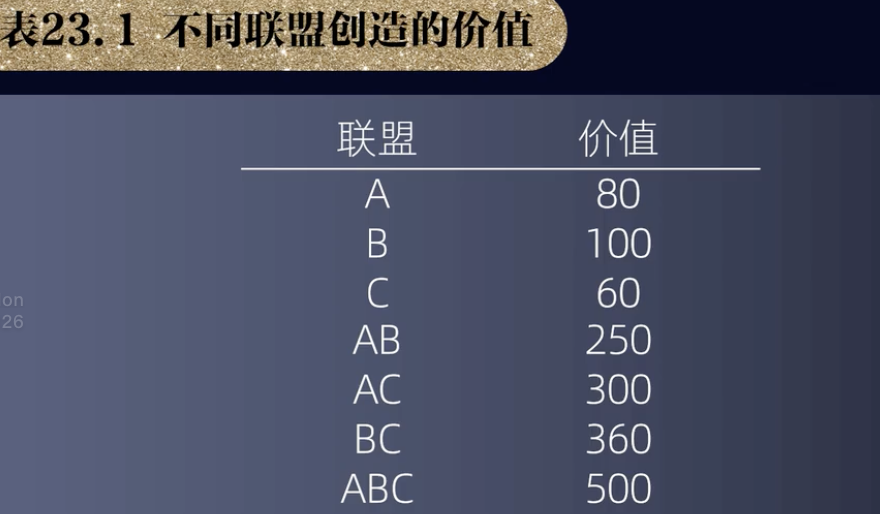
\includegraphics[width=1\textwidth]{./figures/catch2023-08-06-09.46.08.png}
            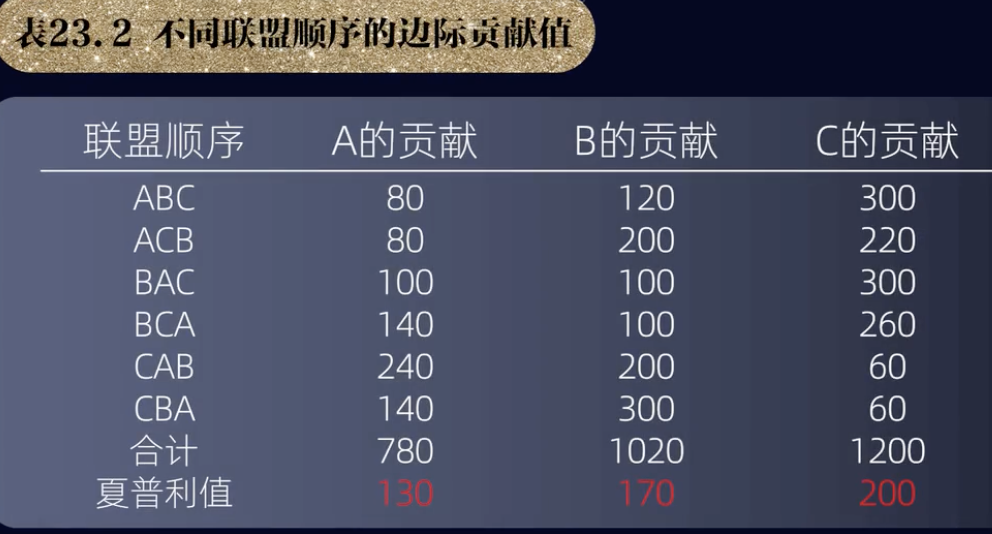
\includegraphics[width=1\textwidth]{./figures/catch2023-08-06-09.52.55.png}
        \end{figure}


        \[\phi_i(n,v) = \frac{1}{n!} \sum_{S \subseteq N \setminus {i}} \binom{n-1}{|S|} [v(S \cup {i}) - v(S)]\]

        通过夏普利值,我们可以发现一个人本身的能力,并不能很好体现出他对团体的贡献,需要通过计算其对团体的边际贡献,才能更好的来评价他对团队的价值。
        为什么用最好上车者价值来计算一个人对团队的贡献,这是因为当一个人威胁要离开团队的时候,其可以从团队获取的最大利益,那就是他的最后上车价值。\par

        大公司往往通过扩大经营规模,创造出很高的总价值,但每个人的这个最后上车价值却不高,那么这样的话,大公司就不会为了挽留某个员工,而付出太大代价,
        每个员工离开,几乎都不会影响组织的正常运行,因为离开会降低其预期收入(店大欺客,客大欺店)。





















    \end{CJK*}
\end{document}
